%===============================================================================
% Zentrale Layout-Angaben und Befehle
%===============================================================================
%
% Für bessere Sicht von falschen Umbrüchen die Option draft benutzen.
% Dadurch können aber die eingebundenen Bilder nicht sichtbar sein.
\documentclass[a4paper, 12pt]{article}
%
% Hier zunächst die benötigten Packages
\usepackage[utf8]{inputenc}
\usepackage[italian]{babel}
\usepackage{fancyhdr}
\usepackage[T1]{fontenc}
\usepackage{ae}
\usepackage{listings}
\usepackage{color}
\usepackage{listings}
\usepackage{wrapfig}
\usepackage[printonlyused]{acronym}
\usepackage{url}
\usepackage{hyperref}
\usepackage{bm}


\usepackage{amsmath}
%
% Einbindung des Grafik-Pakets
\ifx\pdfoutput\undefined
	\usepackage[dvips]{graphicx}
\else
	\usepackage[pdftex]{graphicx}
\pdfcompresslevel=9
\pdfpageheight=297mm
\pdfpagewidth=210mm
\fi
%
% Page-Layout
\setlength\headheight{14pt}
\setlength\topmargin{-15,4mm}
\setlength\oddsidemargin{-0,4mm}
\setlength\evensidemargin{-0,4mm}
\setlength\textwidth{160mm}
\setlength\textheight{252mm}
%
% Absatzeinstellungen
\setlength\parindent{0mm}
\setlength\parskip{2ex}
%
% Kopf- und Fusszeile
\pagestyle{fancy}
\fancyhf{} % alles löschen
\fancyhead[LO]{\footnotesize\sc\nouppercase{\leftmark}}
\fancyfoot[LO]{\footnotesize\sc }
\fancyfoot[RO]{\thepage}
\renewcommand{\headrulewidth}{0pt}
\renewcommand{\footrulewidth}{0pt}
%
% Bessere Fehlermeldungen
\errorcontextlines=999
%
% Anweisung zur Erstellung der Titelseite
% #1 Bachelorarbeit || Masterarbeit
% #2 = Studiengang
% #3 = Titel der Arbeit
% #4 = Autor
% #5 = Abgabedatum
\renewcommand{\maketitle}[5]
{
\pagenumbering{Alph}
%\begin{titlepage}
%\centering
%\begin{minipage}[t]{16cm}
%\begin{minipage}{3cm}
%    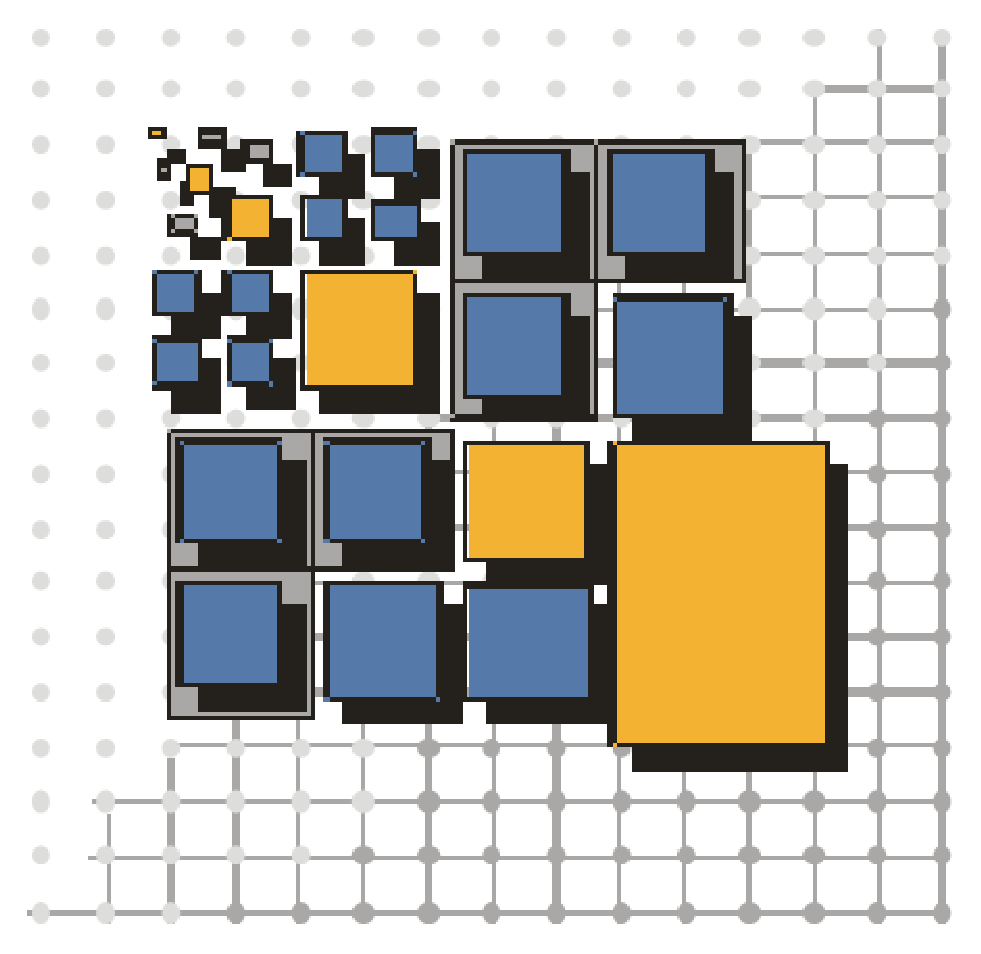
\includegraphics[height=26mm]{includes/vs-logo}
%\end{minipage}
%\hfill
%\begin{minipage}{9cm}
%  \centering
%    Otto-Friedrich-Universität Bamberg\\[12pt]
%    {\Large Lehrstuhl für Praktische Informatik}
%\end{minipage}
%\hfill
%\begin{minipage}{3cm}
%    
\includegraphics[height=26mm]{includes/UB-Logo-neu_blau-cmyk}
%\end{minipage}
%\end{minipage}\\[130pt]
%{\LARGE #1}\\[24pt]
%im Studiengang #2\\
%der Fakultät Wirtschaftsinformatik und Angewandte Informatik\\
%der Otto-Friedrich-Universität Bamberg\\[90pt]
%Zum Thema:\\[24pt]
%{\Huge #3}\\[60pt]
%\vfill
%\begin{minipage}{\textwidth}
%\center
%Vorgelegt von:\\
%{\Large #4\\[12pt]}
%Themensteller:\\
%Prof. Dr. Guido Wirtz\\[12pt]
%Abgabedatum:\\
%#5\\
%\end{minipage}
%\end{titlepage}
\begin{titlepage}
%
%
% ONCE YOU ARE FINISHED WITH YOUR CHANGES MODIFY "RED" WITH "BLACK" IN ALL \textcolor COMMENTS
%
%
\begin{center}
{{\Large{\textsc{Alma Mater Studiorum $\cdot$ Università di  Bologna}}}} 
\rule[0.1cm]{15.8cm}{0.1mm}
\rule[0.5cm]{15.8cm}{0.6mm}
\\\vspace{6mm}
{\small{\bf Scuola di Scienze \\
Dipartimento di Fisica e Astronomia\\
Tesi triennale in Fisica}}
\end{center}

\vspace{23mm}

\begin{center}\textcolor{red}{
%
% INSERT THE TITLE OF YOUR THESIS
%
{\LARGE{\bf APPLICAZIONI DEL MACHINE LEARNING ALLA FISICA DELLE ALTE ENERGIE}}\\
}\end{center}

\vspace{50mm} \par \noindent

\begin{minipage}[t]{0.47\textwidth}
%
% INSERT THE NAME OF THE SUPERVISOR WITH ITS TITLE (DR. OR PROF.)
%
{\large{\bf Supervisor: \vspace{2mm}\\\textcolor{red}{
Prof./Dr. Name Surname}\\\\
%
% INSERT THE NAME OF THE CO-SUPERVISOR WITH ITS TITLE (DR. OR PROF.)
%
% IF THERE ARE NO CO-SUPERVISORS REMOVE THE FOLLOWING 5 LINES
%
\textcolor{red}{
\bf Co-supervisor: (optional)
\vspace{2mm}
Prof./Dr. Name Surname\\\\}}}
\end{minipage}
%
\hfill
%
\begin{minipage}[t]{0.47\textwidth}\raggedleft \textcolor{black}{
{\large{\bf Submitted by:
\vspace{2mm}\\
%
% INSERT THE NAME OF THE GRADUAND
%
\textcolor{red}{
Schiazza Filippo Antonio}}}
}
\end{minipage}

\vspace{40mm}

\begin{center}
%
% INSERT THE ACADEMIC YEAR
%
Anno accademico 2019/2020
\end{center}

\end{titlepage}
}
%
% Anweisung zur Erstellung der Eigenständigkeitserklärung
% #1 = Typ der Arbeit
% #2 = Datum
% #3 = Vorname Name
\newcommand{\makedeclaration}[3]
{
	\fancyhead[LO]{\footnotesize\sc\nouppercase{Eigenständigkeitserklärung}}
	%
			\vspace*{18cm}
			Ich erkläre hiermit gemäß §17 Abs. 2 APO, dass ich die vorstehende #1 selbstständig verfasst 
			und keine anderen als die angegebenen Quellen und Hilfsmittel verwendet habe.\\
			\vspace*{1cm}
			
			Bamberg, den #2 \hspace{5cm} #3
	%
}
%
% Wird für Hintergrund von Codelistings benötigt
\definecolor{hellgrau}{gray}{0.9}
%
% Einstellungen für Java-Code
\lstdefinestyle{javaStyle}{%
  basicstyle=\small,%
  backgroundcolor=\color{hellgrau},%
  keywordstyle=\bfseries,%
  showstringspaces=false,%
  language=Java,%
  numbers=left,%
  numberstyle=\tiny,%
  stepnumber=1,%
  numbersep=5pt,%
  extendedchars=true,%
  xleftmargin=2em,%
  lineskip=-1pt,%
  breaklines%
}
%
% neues environment für Java-Sourcecode
% #1 = "caption={Hier eigene Überschrift}, label={Hier eigenes Label}"
\lstnewenvironment{javacode}[1][]{%
\lstset{style=javaStyle,#1}%
}{}
%
% Befehl zum Einbinden von Java-Sourcecode aus Datei
% #1 = Dateiname relativ zu src-Verzeichnis
% #2 = Überschrift
% #3 = Label
\newcommand{\javafile}[3]{%
   \lstinputlisting[%
     caption={#2},%
     label={#3},%
     style=javaStyle]{src/#1}%
}
%
% Einbindung eines Bildes
% #1 = label für \ref-Verweise
% #2 = Name des Bildes ohne Endung relativ zu images-Verzeichnis
% #3 = Beschriftung
% #4 = Breite des Bildes im Dokument in cm
\newcommand{\bild}[4]{%
  \begin{figure}[htb]%
    \begin{center}%
      \includegraphics[width=#4cm]{images/#2}%
      \vskip -0.3cm%
      \caption{#3}%
      \vskip -0,2cm%
      \label{#1}%
    \end{center}%
  \end{figure}%
}
%
% Umgebung für Fliesstext um Grafik
% #1 = Ausrichtung: r, l, i, ...
% #2 = Breite des Bildes in cm
% #3 = Name des Bildes ohne Endung relativ zu images-Verzeichnis
% #4 = Beschriftung
% #5 = label für \ref-Verweise
\newcommand{\fliesstext}[5]{%
\begin{wrapfigure}{#1}{#2cm}%
\includegraphics[width=#2cm]{images/#3}%
\caption{#4}%
\label{#5}%
\end{wrapfigure}%
}
%%% Local Variables:
%%% mode: latex
%%% TeX-master: t
%%% End:
